\documentclass[12pt,a4paper]{report}
\usepackage[utf8]{inputenc}
\usepackage{titlesec}
\usepackage{graphicx}
\usepackage[utf8]{inputenc}
\usepackage[dvipsnames]{xcolor}
\usepackage{color}
\usepackage{imakeidx}
\usepackage[T1]{fontenc}
\usepackage{listings}
\usepackage{fancybox, calc} 
\usepackage{hyperref}
\usepackage{amssymb}
\usepackage{keystroke}
\usepackage{tikz}


\newtheorem{definition}{Definition} 

\makeindex
\titleformat{\chapter}[hang]{\normalfont\huge\bfseries}{\chaptertitlename\ \thechapter:}{1em}{} 

% Definició dels colors ---------------------------------------------
\definecolor{codegreen}{rgb}{0,0.6,0}
\definecolor{codegray}{rgb}{0.5,0.5,0.5}
\definecolor{codepurple}{rgb}{0.58,0,0.82}
\definecolor{backcolour}{rgb}{0.95,0.95,0.92}

% Definició de l'estil del codi 
\lstdefinestyle{mystyle}{
    backgroundcolor=\color{backcolour},   
    commentstyle=\color{codegreen},
    keywordstyle=\color{magenta},
    numberstyle=\tiny\color{codegray},
    stringstyle=\color{codepurple},
    basicstyle=\footnotesize,
    breakatwhitespace=false,         
    breaklines=true,                 
    captionpos=b,                    
    keepspaces=true,                 
    numbers=left,                    
    numbersep=5pt,                  
    showspaces=false,                
    showstringspaces=false,
    showtabs=false,                  
    tabsize=2
}
\lstset{style=mystyle}


% VARIABLES 
\def \w{$\omega$}
\def \dfa{$FXBP_{DFA} $}
\def \alphabetDFA{$\Sigma$*\dfa}
\def \nfa{$FXBP_{NFA} $}
\def \pfa{$GGR_{PDA} $}
\def \tm{$MSP_{TM} $}
\def \context{$\Phi$}
\def \contextDFA{$\Phi_{DFA}$}
\def \pre{$\Upsilon$}
\def \preDFA{$\Upsilon_{DFA}$}
\def \post{$\Psi$}
\def \postDFA{$\Psi_{DFA}$}
\def \llesca{$\gamma$}


\begin{document}

% Títol de la pràctica -----------------------------------------------
\begin{titlepage}
	\centering
	\includegraphics[width=0.55\textwidth]{udg_logo.png}\par\vspace{1cm}
	{\scshape\LARGE Universitat de girona \par}
	\vspace{1cm}
	{\scshape\Large Pràctica final\par}
	\vspace{1.5cm}
	{\huge\bfseries Fonaments de la computació\par}
	\vspace{2cm}
	{\Large\itshape Francesc Xavier Bullich Parra\par}
	{\Large\itshape Gil Gassó Rovira\par}
	{\Large\itshape Marc Sànchez Pifarré\par}
			
	\vfill
	Tutor de la pràctica\par
	Jaume Rigau

	\vfill

% Bottom of the page
	{\large \today\par}
\end{titlepage}

% Índex -----------------------------------------------
\tableofcontents
\clearpage


\chapter{Introducció}
\setcounter{chapter}{1}

\section{Definicions}

Es defineixen una série de noms que seran utilitzats al llarc de la pràctica per ajudar a la simplificació i l'enteniment de la mateixa. 

\begin{itemize}
\item Definim \dfa{} com l’autòmata finit determinista capaç de reconéixer el llenguatge L(\dfa{}).
\item Definim L (\dfa{}) com el conjunt infinit de mots \w{} que accepta \dfa{}
\item Definim \w{} com un mot tal que \w{} $\in$ L(\dfa{})
\item Definim \alphabetDFA{} com el conjunt de símbols amb el que es construeix el llenguatge L(\dfa{})
\item Definim context \context{} com l’escenari ideal en el que l’autòmata a dissenyar es comportarà de manera correcta, \context{} = < \pre{}, \post{} >  
\item Definim \pre{} com la precondició que s'ha de complir al utilitzar els nostres autòmates. 
\item Definim \post{} com la postcondició de l'autómata.
\end{itemize}

\chapter{Autòmata Finit}

\section{Definició del context}

Sigui \contextDFA{} l'espai de funcionament lògic del nostre autòmata com l'espai estipulat a la Secció 3.Patrons[2]. Per tant acabem d'aquirir totes les definicions assumides a l'enunciat del problema, veure [2].

\textbf{Fem les següents afirmacions sobre \pre{} :}
\begin{itemize}
\item \w{} $\in$ $P_0$ $\wedge$ $P_0$ $\in$ $P$
\item \llesca{} com a llesca continguda dins d'un $P$ on \llesca{} $\in$ \w $\vee$ \llesca{} = $\epsilon$
\end{itemize}

\textbf{Fem les següents afirmacions sobre \post{} :}
\begin{itemize}
\item retorna True quan \dfa{} Accepta \w{} $\leftrightarrow$ $\exists$ \llesca{} $\in$ $P$ que compleix PIP.
\item retorna False quan $\nexists$ \llesca{} $\in$ $P$ que compleix PIP. 
\end{itemize}
on : PIP és la propietat dels patrons implícits parcials definida a [2] apartat 3.3.1. 

\section{Dissenyant el nostre autòmata finit}

Primerament cal observar possibles propietats del problema que ens puguin servir per a la construcció de l’autòmata.

\begin{itemize}
\item Definim 4+ com la seqüència de símbols ‘++++’ d’un mot \w{} comprés dins del llenguatge L(\dfa{}).
\end{itemize}

\textbf{Realitzem les següents observacions :}

\begin{enumerate}
\item Abans i després de la seqüència 4+ hi pot haver qualsevol símbol 0 o més vegades comprés dins de \alphabetDFA{}.
\item Aïllada és la seqüència de simbols ‘-+-’ dins de \w{}
\item Entre dues seqüències 4+ hi trobem 3 aïllades. 
\item 2 aïllades poden compartir el symbol inicial o el symbol final o ambdós. 
\item S’accepta ‘-+-+-’ com a dues cèl·lules aïllades on -+ comparteix - amb +-. 
\item S’accepta ‘-+-+-+-’ coma  tres cèl·lules aïllades on -+ comparteix- amb +-+- i -+-+ comparteix - amb +-.
\item Entre 2 aïllades hi pot aparèixer qualsevol combinació de symbols pertanyent a \alphabetDFA{}.
\item El symbol \Return ens fa tornar a començar a cercar el PIP (RESET). 
\end{enumerate}


Dissenyarem doncs l’autòmata per construcció tenint en compte les anteriors propietats. En la construcció del nostre autòmata reduim el problema al tractament d’un subconjunt dels símbols de l’alfabet, concretament es construeix a partir del subconjunt {+,-}, ja que detectem que el símbol \Return actúa com a RESET. La funció del RESET en \dfa{} és exemplificada al capítol 1 del llibre [1], concretament als exemples 1.15 i 1.17.
 
Incorporarem el RESET al nostre disseny a l’últim pas de la construcció.

\textbf{Fem les següents definicions en l’escenari sense RESET :}

\begin{itemize}
\item Definim pa com la seqüència ‘-+’
\item Definim fa com la seqüència ‘+-’
\item Definim l’operació CONCATENACIÓ amb el symbol | 
\item Definim 3aïllades com :
\begin{itemize}
\item ({+-}* | pa | (-{+-}*)* | pa | (-{+-}*)* | pa | - | {+-}*) $\vee$ ({+-}* | - | fa | (-{+-}*)* | fa | (-{+-}*)* | fa | {+-}*)
\end{itemize}
\end{itemize}

Per tant podem concebre que en un entorn on no hi ha RESET es cerca si el mot conté la següent seqüència de simbols : 

\begin{center}
{+-}* | 4+ | 3aïllades | 4+ | {+-}*
\end{center}

\subsection{Construïm l’autòmata sense RESET}

\begin{center}
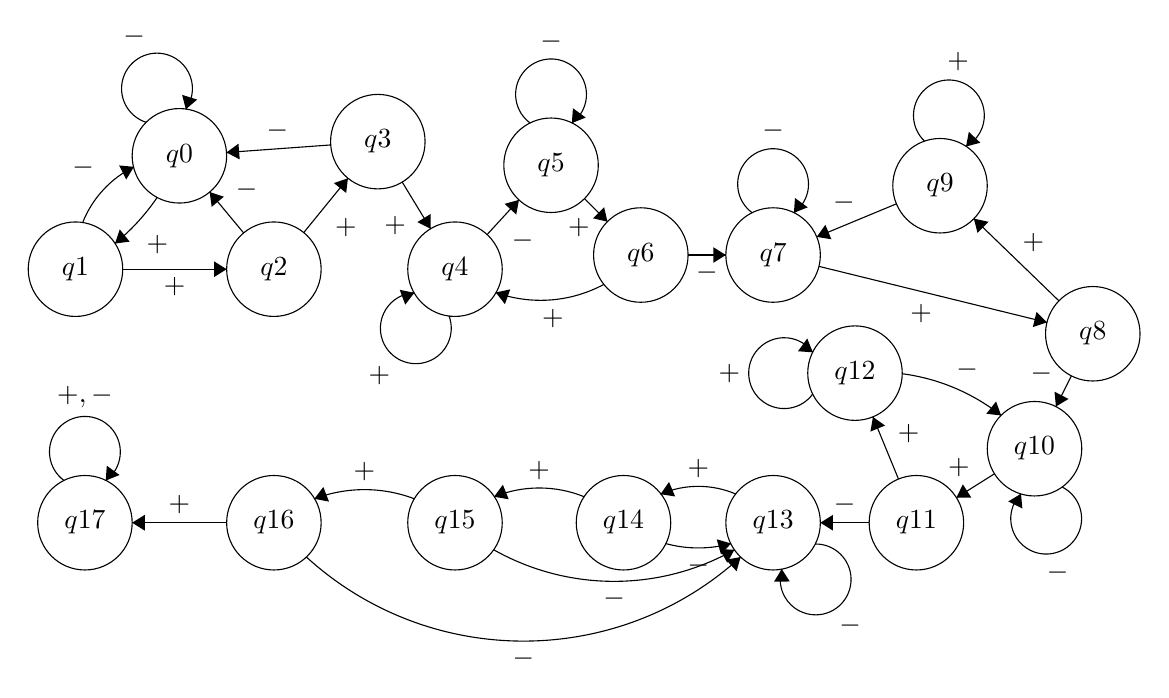
\begin{tikzpicture}[scale=0.2]
\tikzstyle{every node}+=[inner sep=0pt]
\draw [black] (13.9,-8) circle (3);
\draw (13.9,-8) node {$q0$};
\draw [black] (7.3,-15.2) circle (3);
\draw (7.3,-15.2) node {$q1$};
\draw [black] (19.9,-15.2) circle (3);
\draw (19.9,-15.2) node {$q2$};
\draw [black] (26.5,-7.1) circle (3);
\draw (26.5,-7.1) node {$q3$};
\draw [black] (31.4,-15.2) circle (3);
\draw (31.4,-15.2) node {$q4$};
\draw [black] (37.5,-8.6) circle (3);
\draw (37.5,-8.6) node {$q5$};
\draw [black] (43.2,-14.3) circle (3);
\draw (43.2,-14.3) node {$q6$};
\draw [black] (51.6,-14.3) circle (3);
\draw (51.6,-14.3) node {$q7$};
\draw [black] (71.9,-19.3) circle (3);
\draw (71.9,-19.3) node {$q8$};
\draw [black] (62.2,-9.9) circle (3);
\draw (62.2,-9.9) node {$q9$};
\draw [black] (68.2,-26.6) circle (3);
\draw (68.2,-26.6) node {$q10$};
\draw [black] (60.7,-31.3) circle (3);
\draw (60.7,-31.3) node {$q11$};
\draw [black] (56.8,-21.8) circle (3);
\draw (56.8,-21.8) node {$q12$};
\draw [black] (51.6,-31.3) circle (3);
\draw (51.6,-31.3) node {$q13$};
\draw [black] (42.1,-31.3) circle (3);
\draw (42.1,-31.3) node {$q14$};
\draw [black] (31.4,-31.3) circle (3);
\draw (31.4,-31.3) node {$q15$};
\draw [black] (19.9,-31.3) circle (3);
\draw (19.9,-31.3) node {$q16$};
\draw [black] (7.9,-31.3) circle (3);
\draw (7.9,-31.3) node {$q17$};
\draw [black] (12.49,-10.641) arc (-34.29411:-50.72679:13.88);
\fill [black] (9.81,-13.57) -- (10.74,-13.45) -- (10.11,-12.67);
\draw (11.79,-13.66) node [right] {$+$};
\draw [black] (11.798,-5.876) arc (252.43495:-35.56505:2.25);
\draw (11.02,-1.07) node [above] {$-$};
\fill [black] (14.31,-5.04) -- (15.03,-4.43) -- (14.07,-4.13);
\draw [black] (10.3,-15.2) -- (16.9,-15.2);
\fill [black] (16.9,-15.2) -- (16.1,-14.7) -- (16.1,-15.7);
\draw (13.6,-15.7) node [below] {$+$};
\draw [black] (21.8,-12.87) -- (24.6,-9.43);
\fill [black] (24.6,-9.43) -- (23.71,-9.73) -- (24.49,-10.36);
\draw (23.76,-12.58) node [right] {$+$};
\draw [black] (28.05,-9.67) -- (29.85,-12.63);
\fill [black] (29.85,-12.63) -- (29.86,-11.69) -- (29.01,-12.21);
\draw (28.31,-12.42) node [left] {$+$};
\draw [black] (33.44,-13) -- (35.46,-10.8);
\fill [black] (35.46,-10.8) -- (34.55,-11.05) -- (35.29,-11.73);
\draw (34.98,-13.36) node [right] {$-$};
\draw [black] (39.62,-10.72) -- (41.08,-12.18);
\fill [black] (41.08,-12.18) -- (40.87,-11.26) -- (40.16,-11.97);
\draw (39.26,-11.93) node [below] {$+$};
\draw [black] (36.177,-5.92) arc (234:-54:2.25);
\draw (37.5,-1.35) node [above] {$-$};
\fill [black] (38.82,-5.92) -- (39.7,-5.57) -- (38.89,-4.98);
\draw [black] (40.865,-16.159) arc (-61.6184:-109.65845:8.47);
\fill [black] (33.99,-16.68) -- (34.57,-17.42) -- (34.91,-16.48);
\draw (37.61,-17.72) node [below] {$+$};
\draw [black] (46.2,-14.3) -- (48.6,-14.3);
\fill [black] (48.6,-14.3) -- (47.8,-13.8) -- (47.8,-14.8);
\draw (47.4,-14.8) node [below] {$-$};
\draw [black] (50.277,-11.62) arc (234:-54:2.25);
\draw (51.6,-7.05) node [above] {$-$};
\fill [black] (52.92,-11.62) -- (53.8,-11.27) -- (52.99,-10.68);
\draw [black] (54.51,-15.02) -- (68.99,-18.58);
\fill [black] (68.99,-18.58) -- (68.33,-17.91) -- (68.09,-18.88);
\draw (61,-17.38) node [below] {$+$};
\draw [black] (69.75,-17.21) -- (64.35,-11.99);
\fill [black] (64.35,-11.99) -- (64.58,-12.9) -- (65.28,-12.19);
\draw (68.13,-14.12) node [above] {$+$};
\draw [black] (59.43,-11.05) -- (54.37,-13.15);
\fill [black] (54.37,-13.15) -- (55.3,-13.3) -- (54.92,-12.38);
\draw (56.1,-11.59) node [above] {$-$};
\draw [black] (61.224,-7.075) arc (226.78987:-61.21013:2.25);
\draw (63.35,-2.61) node [above] {$+$};
\fill [black] (63.85,-7.41) -- (64.76,-7.17) -- (64.03,-6.48);
\draw [black] (70.54,-21.98) -- (69.56,-23.92);
\fill [black] (69.56,-23.92) -- (70.36,-23.44) -- (69.47,-22.98);
\draw (69.36,-21.83) node [left] {$-$};
\draw [black] (65.66,-28.19) -- (63.24,-29.71);
\fill [black] (63.24,-29.71) -- (64.19,-29.71) -- (63.65,-28.86);
\draw (63.39,-28.45) node [above] {$+$};
\draw [black] (59.56,-28.52) -- (57.94,-24.58);
\fill [black] (57.94,-24.58) -- (57.78,-25.51) -- (58.71,-25.13);
\draw (59.49,-25.64) node [right] {$+$};
\draw [black] (59.793,-21.838) arc (82.58376:51.74893:12.833);
\fill [black] (66.08,-24.49) -- (65.76,-23.6) -- (65.14,-24.38);
\draw (63.92,-22.22) node [above] {$-$};
\draw [black] (57.7,-31.3) -- (54.6,-31.3);
\fill [black] (54.6,-31.3) -- (55.4,-31.8) -- (55.4,-30.8);
\draw (56.15,-30.8) node [above] {$-$};
\draw [black] (54.12,-23.123) arc (-36:-324:2.25);
\draw (49.55,-21.8) node [left] {$+$};
\fill [black] (54.12,-20.48) -- (53.77,-19.6) -- (53.18,-20.41);
\draw [black] (54.266,-32.65) arc (90.8699:-197.1301:2.25);
\draw (56.49,-37.2) node [below] {$-$};
\fill [black] (52.15,-34.24) -- (51.66,-35.04) -- (52.66,-35.03);
\draw [black] (44.451,-29.486) arc (113.41059:66.58941:6.038);
\fill [black] (44.45,-29.49) -- (45.38,-29.63) -- (44.99,-28.71);
\draw (46.85,-28.49) node [above] {$+$};
\draw [black] (33.885,-29.654) arc (112.1939:67.8061:7.585);
\fill [black] (33.88,-29.65) -- (34.81,-29.81) -- (34.44,-28.89);
\draw (36.75,-28.59) node [above] {$+$};
\draw [black] (22.472,-29.783) arc (110.89771:69.10229:8.911);
\fill [black] (22.47,-29.78) -- (23.4,-29.96) -- (23.04,-29.03);
\draw (25.65,-28.7) node [above] {$+$};
\draw [black] (16.9,-31.3) -- (10.9,-31.3);
\fill [black] (10.9,-31.3) -- (11.7,-31.8) -- (11.7,-30.8);
\draw (13.9,-30.8) node [above] {$+$};
\draw [black] (6.577,-28.62) arc (234:-54:2.25);
\draw (7.9,-24.05) node [above] {$+,-$};
\fill [black] (9.22,-28.62) -- (10.1,-28.27) -- (9.29,-27.68);
\draw [black] (7.749,-12.259) arc (-201.4719:-243.54899:6.719);
\fill [black] (11.01,-8.7) -- (10.07,-8.61) -- (10.52,-9.51);
\draw (8.51,-8.72) node [left] {$-$};
\draw [black] (17.98,-12.9) -- (15.82,-10.3);
\fill [black] (15.82,-10.3) -- (15.95,-11.24) -- (16.72,-10.6);
\draw (17.45,-10.16) node [right] {$-$};
\draw [black] (23.51,-7.31) -- (16.89,-7.79);
\fill [black] (16.89,-7.79) -- (17.73,-8.23) -- (17.65,-7.23);
\draw (20.12,-7) node [above] {$-$};
\draw [black] (31.02,-18.164) arc (20.42917:-267.57083:2.25);
\draw (26.6,-21.32) node [below] {$+$};
\fill [black] (28.82,-16.7) -- (27.89,-16.51) -- (28.24,-17.45);
\draw [black] (69.945,-29.026) arc (63.46232:-224.53768:2.25);
\draw (69.67,-33.84) node [below] {$-$};
\fill [black] (67.34,-29.46) -- (66.53,-29.95) -- (67.43,-30.4);
\draw [black] (48.927,-32.621) arc (-74.6612:-105.3388:7.85);
\fill [black] (48.93,-32.62) -- (48.02,-32.35) -- (48.29,-33.31);
\draw (46.85,-33.4) node [below] {$-$};
\draw [black] (49.539,-33.476) arc (-47.64801:-132.35199:20.468);
\fill [black] (49.54,-33.48) -- (48.61,-33.65) -- (49.28,-34.38);
\draw (35.75,-39.32) node [below] {$-$};
\draw [black] (49.145,-33.016) arc (-60.58176:-119.41824:15.564);
\fill [black] (49.14,-33.02) -- (48.2,-32.97) -- (48.69,-33.84);
\draw (41.5,-35.52) node [below] {$-$};
\end{tikzpicture}
\end{center}





















\begin{multicols}{2}
\end{multicols}







































Un exemple de llesca horitzontal que compleix el patró : 

\begin{lstlisting}[columns=fullflexible]
++++-+-+-+-++++ 
\end{lstlisting}

Un exemple de llesca horitzontal que no compleix el patró : 

\begin{lstlisting}[columns=fullflexible]
++++-+---+-++++ 
\end{lstlisting}

\clearpage

\textcolor{red}{Exemple de codi incrustat en latex}

\lstinputlisting[language=C++, caption=Matrix example]{Matrix.cpp}


\chapter{Push-Down Automata}

\chapter{Turing Machine}

\begin{thebibliography}{9}
\bibitem{FC} 
Fundamental of Computation - Michael Sipser
 
\bibitem{patterns}
\hyperlink{http://ima.udg.edu/~rigau/FC/FC_patterns.pdf}{Problema Patterns (i.e., Cerca de Patrons) - Jaume Rigau} 

\end{thebibliography}

\printindex
\end{document}
